%!TEX root=../robocert.tex
\begin{figure}
	\centering
	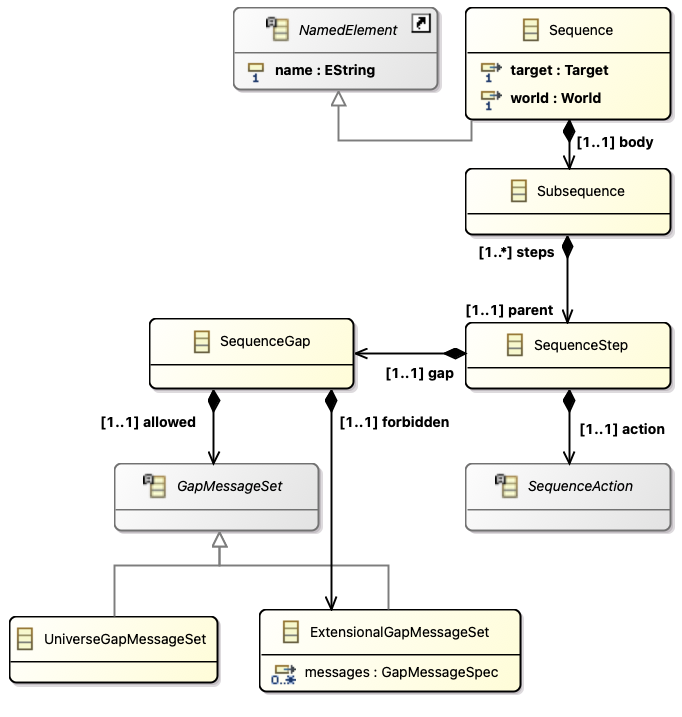
\includegraphics[width=0.7\textwidth]{diagrams/sequences.png}
	\caption{Class diagram for the part of the \langname{} metamodel dealing with sequences.}
	\label{fig:metamodel-sequences}
\end{figure}

\Cref{fig:metamodel-sequences} depicts the part of the metamodel concerning
sequence diagrams and their high-level structure.

\subsection{\msequence}

A \msequence{} represents a sequence diagram.  It is a \mnamedelement{}
that contains:

\begin{itemize}
\item
	a \msubsequence{} (\cref{ssec:metamodel-sequences-subsequences})
	containing the body of the diagram;
\item
	two \mactor s (\cref{sec:metamodel-actors}):
	a \mtarget{} (\cref{ssec:metamodel-actors-target})
	and a \mworld{} (\cref{ssec:metamodel-actors-world}).
\end{itemize}

\begin{lstlisting}[style=Example]
sequence Example
  for module AModule as M,  // RCModuleTarget actor
      world          as W   // World actor
{
    anything until end  // Subsequence
}
\end{lstlisting}

\subsection{\msubsequence}\label{ssec:metamodel-sequences-subsequences}

A \msubsequence{} is a sequential composition of one or more \msequencestep s
(\cref{ssec:metamodel-sequences-steps}).
All \msequence s contain exactly one \msubsequence{} at the top level, but
may contain multiple nested \msubsequence s introduced by constructs such as
\mloopaction s.

\begin{lstlisting}[style=Example]
{
    anything until operation O1() from M to W  // SequenceStep
then
    operation O2() from M to W                 // SequenceStep
then
    end                                        // SequenceStep
}
\end{lstlisting}

\subsection{\msequencestep}\label{ssec:metamodel-sequences-steps}

A \msequencestep{} is a single step in a \msubsequence.  It consists of a
\msequencegap{} (\cref{ssec:metamodel-sequences-gaps}) and a
\msequenceaction{} (\cref{sec:metamodel-actions}).

\begin{lstlisting}[style=Example]
anything until operation O() from M to W
// SequenceStep with explicit SequenceGap and SequenceAction

operation O() from M to W
// SequenceStep with explicit SequenceAction only;
// implicit SequenceGap with empty allow set
\end{lstlisting}

\subsection{\msequencegap}\label{ssec:metamodel-sequences-gaps}

A \msequencegap{} represents a condition on any
communication\footnote{In PSCs, this would correspond to
  \emph{intraMSG}s.} that can happen \emph{before} a \msequenceaction.
It contains two \mmessageset s (\cref{ssec:metamodel-messages-sets}):
one specifying the messages \emph{allowed} to pass inside the gap, and
another specifying the messages \emph{forbidden} to pass.

\begin{lstlisting}[style=Example]
anything
    in     { operation O1() from M to W   // allowed ExtensionalMessageSet
           , operation O2() from M to W }
    // a UniverseMessageSet is implied for the allow set
    // if 'in {..}' is omitted;

    except { operation O2() from M to W } // forbidden ExtensionalMessageSet
    // an empty ExtensionalMessageSet is implied for the forbidden set
    // if 'except {..}' is omitted
until // only permits O1
\end{lstlisting}

